
%%%%%%%%%%%%%%%%%%%%%%%%%%%%%%%%%%%%%%%%%%%%%%%%%%%%%%%%%%%%%%%%%%%%%%%%%%%%%%
% Copyright (c) 2003-2018 by The University of Queensland
% http://www.uq.edu.au
%
% Primary Business: Queensland, Australia
% Licensed under the Apache License, version 2.0
% http://www.apache.org/licenses/LICENSE-2.0
%
% Development until 2012 by Earth Systems Science Computational Center (ESSCC)
% Development 2012-2013 by School of Earth Sciences
% Development from 2014 by Centre for Geoscience Computing (GeoComp)
%
%%%%%%%%%%%%%%%%%%%%%%%%%%%%%%%%%%%%%%%%%%%%%%%%%%%%%%%%%%%%%%%%%%%%%%%%%%%%%%

The acoustic wave equation governs the propagation of pressure waves. Wave
types that obey this law tend to travel in liquids or gases where shear waves
or longitudinal style wave motion is not possible. An obvious example is sound
waves.

The acoustic wave equation is defined as;
\begin{equation}
 \nabla ^2 p - \frac{1}{c^2} \frac{\partial ^2 p}{\partial t^2} = 0
\label{eqn:acswave}
\end{equation}
where $p$ is the pressure, $t$ is the time and $c$ is the wave velocity. In this
chapter the acoustic wave equation is demonstrated. Important steps include the
translation of the Laplacian $\nabla^2$ to the \esc general form, the stiff
equation stability criterion and solving for the displacement or acceleration solution.

\section{The Laplacian in \esc}
The Laplacian operator which can be written as $\Delta$ or $\nabla^2$,  is
calculated via the divergence of the gradient of the object, which in this
example is the scalar $p$. Thus we can write;
\begin{equation}
 \nabla^2 p = \nabla \cdot \nabla p = 
	\sum_{i}^n
	\frac{\partial^2 p}{\partial x^2_{i}}
 \label{eqn:laplacian}
\end{equation}
For the two dimensional case in Cartesian coordinates \autoref{eqn:laplacian}
becomes;
\begin{equation}
 \nabla^2 p = \frac{\partial^2 p}{\partial x^2} 
		   + \frac{\partial^2 p}{\partial y^2}
\end{equation}

In \esc the Laplacian is calculated using the divergence representation and the
intrinsic functions \textit{grad()} and \textit{trace()}. The function
\textit{grad{}} will return the spatial gradients of an object.  
For a rank 0 solution, this is of the form;
\begin{equation}
 \nabla p = \left[
	   \frac{\partial p}{\partial x _{0}},  
	   \frac{\partial p}{\partial x _{1}}
                  \right]
\label{eqn:grad}
\end{equation}
Larger ranked solution objects will return gradient tensors. For example, a
pressure field which acts in the directions $p _{0}$ and $p
_{1}$ would return;
\begin{equation}
  \nabla p = \begin{bmatrix}
	   \frac{\partial p _{0}}{\partial x _{0}} &
		\frac{\partial p _{1}}{\partial x _{0}} \\
	  \frac{\partial p _{0}}{\partial x _{1}} &
		\frac{\partial p _{1}}{\partial x _{1}} 
                  \end{bmatrix}
\label{eqn:gradrank1}
\end{equation}

\autoref{eqn:grad} corresponds to the Linear PDE general form value
$X$. Notice however, that the general form contains the term $X
_{i,j}$\footnote{This is the first derivative in the $j^{th}$
direction for the $i^{th}$ component of the solution.},
hence for a rank 0 object there is no need to do more then calculate the
gradient and submit it to the solver. In the case of the rank 1 or greater
object, it is also necessary to calculate the trace. This is the sum of the
diagonal in \autoref{eqn:gradrank1}. 

Thus when solving for equations containing the Laplacian one of two things must
be completed. If the object \verb!p! is less than rank 1 the gradient is
calculated via;
\begin{python}
gradient=grad(p)
\end{python}
and if the object is greater then or equal to a rank 1 tensor, the trace of
the gradient is calculated.
\begin{python}
 gradient=trace(grad(p))
\end{python}
These values can then be submitted to the PDE solver via the general form term
$X$. The Laplacian is then computed in the solution process by taking the
divergence of $X$.

Note, if you are unsure about the rank of your tensor, the \textit{getRank}
command will return the rank of the PDE object.
\begin{python}
 rank = p.getRank()
\end{python}


\section{Numerical Solution Stability} \label{sec:nsstab}
Unfortunately, the wave equation belongs to a class of equations called
\textbf{stiff} PDEs. These types of equations can be difficult to solve
numerically as they tend to oscillate about the exact solution, which can
eventually lead to a catastrophic failure. To counter this problem, explicitly
stable schemes like the backwards Euler method, and correct parameterisation of
the problem are required. 

There are two variables which must be considered for
stability when numerically trying to solve the wave equation. For linear media,
the two variables are related via;
\begin{equation} \label{eqn:freqvel}
f=\frac{v}{\lambda}
\end{equation}
The velocity $v$ that a wave travels in a medium is an important variable. For
stability the analytical wave must not propagate faster then the numerical wave
is able to, and in general, needs to be much slower then the numerical wave.
For example, a line 100m long is discretised into 1m intervals or 101 nodes. If
a wave enters with a propagation velocity of 100m/s then the travel time for
the wave between each node will be 0.01 seconds. The time step, must therefore
be significantly less than this. Of the order $10E-4$ would be appropriate. 
This stability criterion is known as the Courant\textendash
Friedrichs\textendash Lewy condition given by
\begin{equation}
dt=f\cdot \frac{dx}{v}
\end{equation}
where $dx$ is the mesh size and $f$ is a safety factor. To obtain a time step of
$10E-4$, a safety factor of $f=0.1$ was used.

The wave frequency content also plays a part in numerical stability. The
Nyquist-sampling theorem states that a signals bandwidth content will be
accurately represented when an equispaced sampling rate $f _{n}$ is
equal to or greater then twice the maximum frequency of the signal
$f_{s}$, or;
\begin{equation} \label{eqn:samptheorem}
 f_{n} \geqslant f_{s}
\end{equation}
For example, a 50Hz signal will require a sampling rate greater then 100Hz or
one sample every 0.01 seconds. The wave equation relies on a spatial frequency,
thus the sampling theorem in this case applies to the solution mesh spacing.
This relationship confirms that the frequency content of the input signal
directly affects the time discretisation of the problem.

To accurately model the wave equation with high resolutions and velocities
means that very fine spatial and time discretisation is necessary for most
problems.  This requirement makes the wave equation arduous to
solve numerically due to the large number of time iterations required in each
solution. Models with very high velocities and frequencies will be the worst
affected by this problem.

\section{Displacement Solution}
\sslist{example07a.py}

We begin the solution to this PDE with the centred difference formula for the
second derivative;
\begin{equation}
 f''(x) \approx \frac{f(x+h - 2f(x) + f(x-h)}{h^2}
\label{eqn:centdiff}
\end{equation}
substituting \autoref{eqn:centdiff} for $\frac{\partial ^2 p }{\partial t ^2}$
in \autoref{eqn:acswave};
\begin{equation}
 \nabla ^2 p - \frac{1}{c^2h^2} \left[p_{(t+1)} - 2p_{(t)} +
p_{(t-1)} \right]
= 0
\label{eqn:waveu}
\end{equation}
Rearranging for $p_{(t+1)}$;
\begin{equation}
 p_{(t+1)} = c^2 h^2 \nabla ^2 p_{(t)} +2p_{(t)} -
p_{(t-1)}
\end{equation}
this can be compared with the general form of the \modLPDE module and it
becomes clear that $D=1$, $X_{i,j}=-c^2 h^2 \nabla ^2 p_{(t)}$ and
$Y=2p_{(t)} - p_{(t-1)}$.

The solution script is similar to others that we have created in previous
chapters. The general steps are;
\begin{enumerate}
 \item The necessary libraries must be imported.
 \item The domain needs to be defined.
 \item The time iteration and control parameters need to be defined.
 \item The PDE is initialised with source and boundary conditions.
 \item The time loop is started and the PDE is solved at consecutive time steps.
 \item All or select solutions are saved to file for visualisation later on.
\end{enumerate}

Parts of the script which warrant more attention are the definition of the
source, visualising the source, the solution time loop and the VTK data export.

\subsection{Pressure Sources}
As the pressure is a scalar, one need only define the pressure for two 
time steps prior to the start of the solution loop. Two known solutions are
required because the wave equation contains a double partial derivative with
respect to time. This is often a good opportunity to introduce a source to the
solution. This model has the source located at it's centre. The source should
be smooth and cover a number of samples to satisfy the frequency stability
criterion. Small sources will generate high frequency signals. Here, when using
a rectangular domain, the source is defined by a cosine function.
\begin{python}
U0=0.01 # amplitude of point source
xc=[500,500] #location of point source
# define small radius around point xc
src_radius = 30
# for first two time steps
u=U0*(cos(length(x-xc)*3.1415/src_radius)+1)*\
	whereNegative(length(x-xc)-src_radius)
u_m1=u
\end{python}

\subsection{Visualising the Source}
There are two options for visualising the source. The first is to export the
initial conditions of the model to VTK, which can be interpreted as a scalar
surface in \mayavi. The second is to take a cross section of the model which
will require the \textit{Locator} function. 
First \verb!Locator! must be imported;
\begin{python}
 from esys.escript.pdetools import Locator
\end{python}
The function can then be used on the domain to locate the nearest domain node
to the point or points of interest.

It is now necessary to build a list of $(x,y)$ locations that specify where are
model slice will go. This is easily implemented with a loop;
\begin{python}
cut_loc=[]
src_cut=[]
for i in range(ndx/2-ndx/10,ndx/2+ndx/10):
    cut_loc.append(xstep*i)
    src_cut.append([xstep*i,xc[1]])
\end{python}
We then submit the output to \verb!Locator! and finally return the appropriate
values using the \verb!getValue! function.
\begin{python}
src=Locator(mydomain,src_cut)
src_cut=src.getValue(u)
\end{python}
It is then a trivial task to plot and save the output using \mpl
(\autoref{fig:cxsource}).
\begin{python}
pl.plot(cut_loc,src_cut)
pl.axis([xc[0]-src_radius*3,xc[0]+src_radius*3,0.,2*U0])
pl.savefig(os.path.join(savepath,"source_line.png"))
\end{python}
\begin{figure}[h]
 \centering
	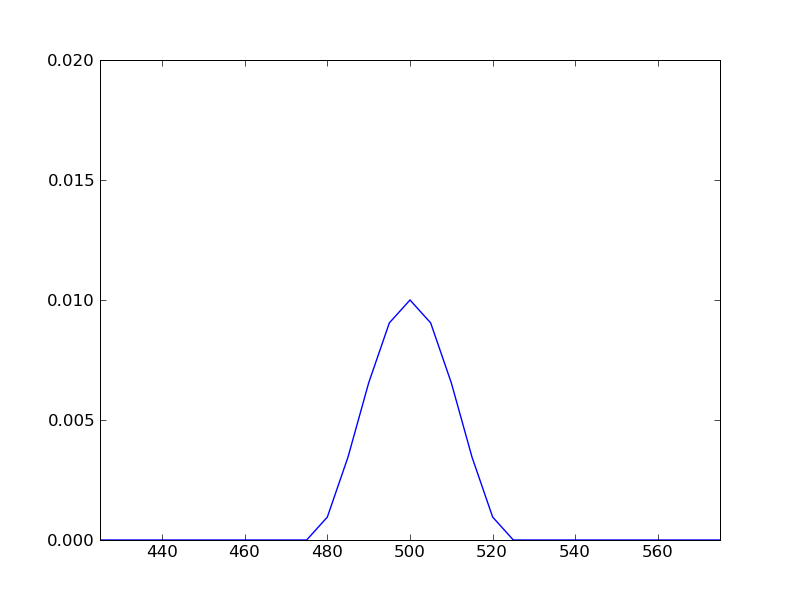
\includegraphics[width=6in]{figures/sourceline.png}
 \caption{Cross section of the source function.}
 \label{fig:cxsource}
\end{figure}


\subsection{Point Monitoring}
In the more general case where the solution mesh is irregular or specific
locations need to be monitored, it is simple enough to use the \textit{Locator}
function. 
\begin{python}
 rec=Locator(mydomain,[250.,250.])
\end{python}
 When the solution \verb u  is updated we can extract the value at that point
via;
\begin{python}
 u_rec=rec.getValue(u)
\end{python}
For consecutive time steps one can record the values from \verb!u_rec! in an
array initialised as \verb!u_rec0=[]! with;
\begin{python}
  u_rec0.append(rec.getValue(u))
\end{python}

It can be useful to monitor the value at a single or multiple individual points
in the model during the modelling process. This is done using 
the \verb!Locator! function.


\section{Acceleration Solution}
\sslist{example07b.py}

An alternative method to the displacement solution, is to solve for the
acceleration $\frac{\partial ^2 p}{\partial t^2}$ directly. The displacement can
then be derived from the acceleration after a solution has been calculated
The acceleration is given by a modified form of \autoref{eqn:waveu};
\begin{equation}
  \nabla ^2 p - \frac{1}{c^2} a = 0
\label{eqn:wavea}
\end{equation}
and can be solved directly with $Y=0$ and $X=-c^2 \nabla ^2 p_{(t)}$.
After each iteration the displacement is re-evaluated via;
\begin{equation}
 p_{(t+1)}=2p_{(t)} - p_{(t-1)} + h^2a
\end{equation}

\subsection{Lumping}
For \esc, the acceleration solution is preferred as it allows the use of matrix
lumping. Lumping or mass lumping as it is sometimes known, is the process of
aggressively approximating the density elements of a mass matrix into the main
diagonal. The use of Lumping is motivated by the simplicity of diagonal matrix
 inversion. As a result, Lumping can significantly reduce the computational
requirements of a problem. Care should be taken however, as this
function can only be used when the $A$, $B$ and $C$ coefficients of the
general form are zero. 

More information about the lumping implementation used in \esc and its accuracy
can be found in the user guide.

To turn lumping on in \esc one can use the command;
\begin{python}
 mypde.getSolverOptions().setSolverMethod(SolverOptions.HRZ_LUMPING)
\end{python}
It is also possible to check if lumping is set using;
\begin{python}
  print(mypde.isUsingLumping())
\end{python}

\section{Stability Investigation}
It is now prudent to investigate the stability limitations of this problem.
First, we let the frequency content of the source be very small. If we define
the source as a cosine input, then the wavlength of the input is equal to the
radius of the source. Let this value be 5 meters. Now, if the maximum velocity
of the model is $c=380.0ms^{-1}$, then the source
frequency is $f_{r} = \frac{380.0}{5} = 76.0 Hz$. This is a worst case
scenario with a small source and the models maximum velocity. 

Furthermore, we know from \autoref{sec:nsstab}, that the spatial sampling
frequency must be at least twice this value to ensure stability. If we assume
the model mesh is a square equispaced grid,
then the sampling interval is the side length divided by the number of samples,
given by $\Delta x = \frac{1000.0m}{400} = 2.5m$ and the maximum sampling
frequency capable at this interval is
$f_{s}=\frac{380.0ms^{-1}}{2.5m}=152Hz$ this is just equal to the
required rate satisfying \autoref{eqn:samptheorem}. 

\autoref{fig:ex07sampth} depicts three examples where the grid has been
undersampled, sampled correctly, and over sampled. The grids used had
200, 400 and 800 nodes per side respectively. Obviously, the oversampled grid
retains the best resolution of the modelled wave.

The time step required for each of these examples is simply calculated from
the propagation requirement. For a maximum velocity of $380.0ms^{-1}$,
\begin{subequations}
 \begin{equation}
  \Delta t \leq \frac{1000.0m}{200} \frac{1}{380.0} = 0.013s
 \end{equation}
 \begin{equation}
  \Delta t \leq \frac{1000.0m}{400} \frac{1}{380.0} = 0.0065s
 \end{equation}
 \begin{equation}
  \Delta t \leq \frac{1000.0m}{800} \frac{1}{380.0} = 0.0032s
 \end{equation}
\end{subequations}
Observe that for each doubling of the number of nodes in the mesh, we halve
the time step. To illustrate the impact this has, consider our model. If the
source is placed at the center, it is $500m$ from the nearest boundary. With a
velocity of $380.0ms^{-1}$ it will take $\approx1.3s$ for the wavefront to
reach that boundary. In each case, this equates to $100$,  $200$ and $400$ time
steps. This is again, only a best case scenario, for true stability these time
values may need to be halved and possibly halved again.

\begin{figure}[ht]
\centering
\subfigure[Undersampled Example]{
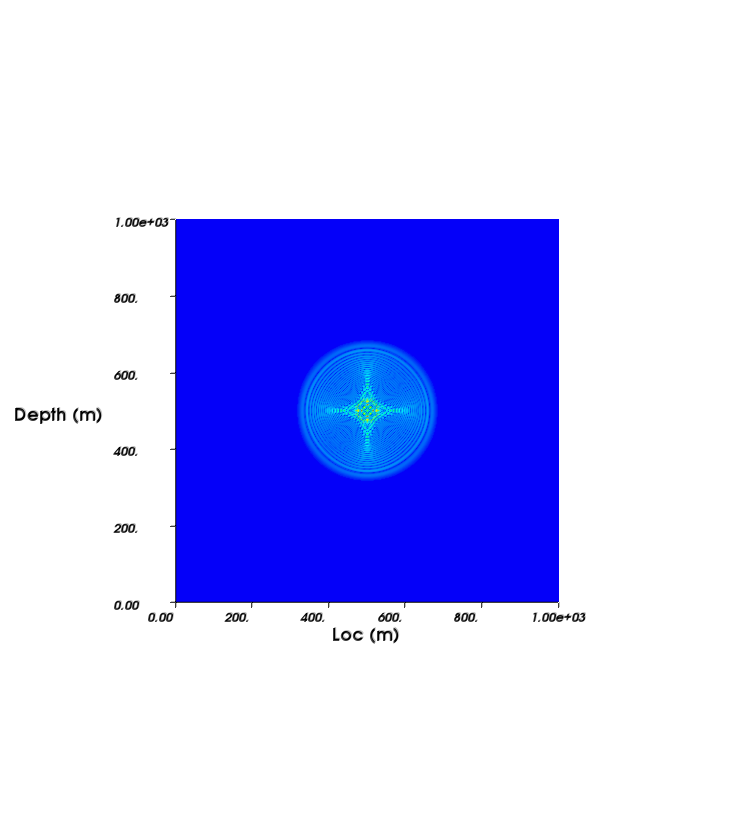
\includegraphics[width=0.45\textwidth,trim=0cm 6cm 5cm 6cm,clip]{figures/ex07usamp.png}
\label{fig:ex07usamp}
}
\subfigure[Just sampled Example]{
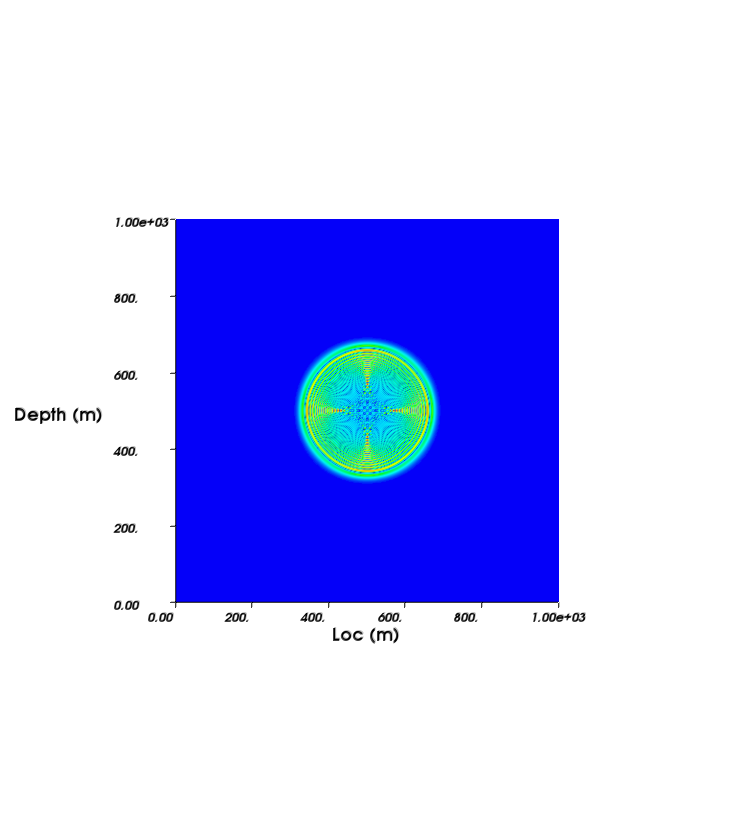
\includegraphics[width=0.45\textwidth,trim=0cm 6cm 5cm 6cm,clip]{figures/ex07jsamp.png}
\label{fig:ex07jsamp}
}
\subfigure[Over sampled Example]{
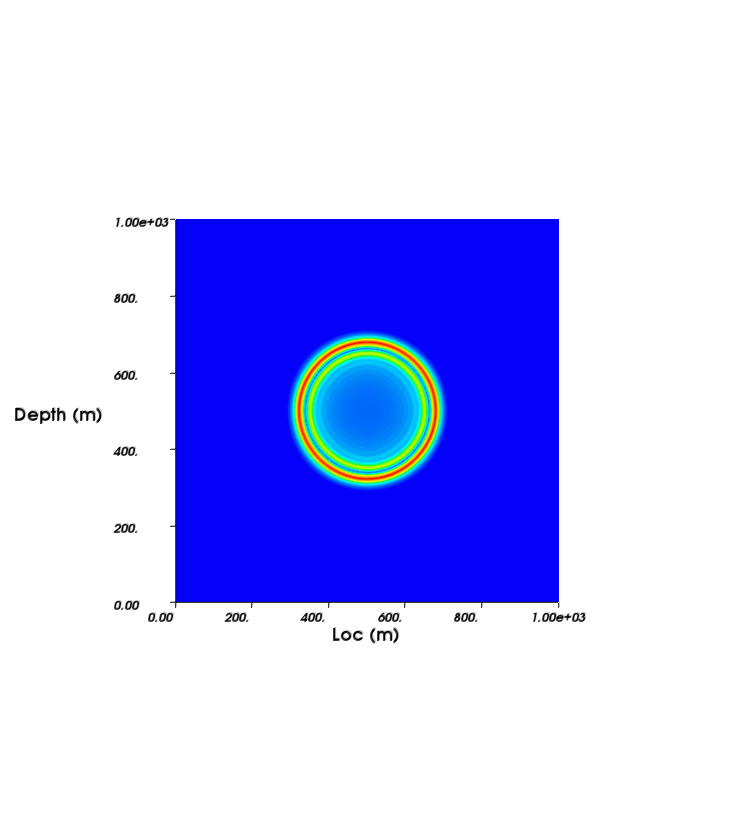
\includegraphics[width=0.45\textwidth,trim=0cm 6cm 5cm 6cm,clip]{figures/ex07nsamp.png}
\label{fig:ex07nsamp}
}
\caption{Sampling Theorem example for stability investigation}
\label{fig:ex07sampth}
\end{figure}

